\subsection{Codi i control de versions}
\label{metodologia:codi_versions}
Per al control de versions del projecte, es fa ús de repositoris \textit{git}\footnote{https://git-scm.com/}, un repositori destinat al \textit{frontend} i un per al \textit{backend}.\\
\newline Els repositoris estan estructurats tal i com s'indica a \textit{gitflow}\footnote{http://nvie.com/posts/a-successful-git-branching-model/}, una estandarització per a l'ús de branques a repositoris principalment git.\\
\begin{figure}[h]
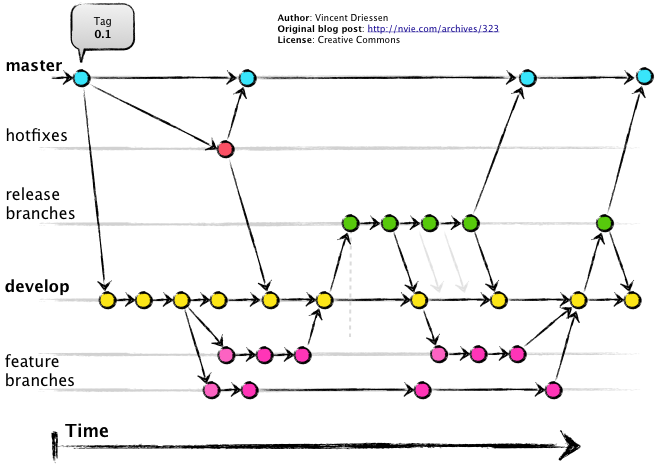
\includegraphics[scale=0.5]{sections/gestio/gitflow.png}
\centering
\caption{Gitflow}
\label{fig:gitflow}
\end{figure}
\clearpage
Internament els repositoris segueixen l'estructura mostrada a la Figura \ref{fig:gitflow}).\\
En essència es pot resumir l'esquema anterior en un repositori amb dues branques principals:
\begin{itemize}
	\item \textbf{Master}: En aquesta branca només hi ha codi plenament funcional i testejat. El codi que aquí es troba, està preparat per a ser publicat en qualsevol moment.
	\item \textbf{Develop}: La branca de desenvolupament. El codi que aquí es trobi, també haurà d'estar testejat i ésser funcional, però el grau de rigurositat d'aquesta branca és menor que a \textit{master}.
\end{itemize}
Partint d'aquestes branques inicials, a mesura que avanci el projecte es creuran noves branques a partir de la branca \textit{develop}, mai desde \textit{master}. A \textit{master} només s'hi passarà el codi que des de la branca \textit{develop} es consideri apte.\\
\newline Les branques es crearan a partir de les tasques definides a la secció \ref{gestio:tasques},
el nom de les branques ve donat pel programari de gestió de tasques que es fa servir (a la secció \nameref{metodologia:software_suport} es donen detalls del programari emprat), ja que d'aquesta forma queden vinculades les tasques amb els \textit{commits} i les branques.\\
\newline A nivell d'equip, les dinàmiques són senzilles.
\begin{itemize}
    \item Cada tasca en una branca.
    \item Un cop acabada la tasca, es porten els canvis cap a la branca \textit{develop}.
    \item En cas d'haver de solucionar errors sobre \textit{master} es farà creant branques amb el l'etiqueta \textit{bugfix}.
    \item Cada cop que una tasca es doni per finalitzada i validada, s'elimina la branca.
\end{itemize}
\subsubsection{TDD}
\label{metodologia:tdd}
Rep el nom de \textit{TDD}\footnote{Test-Driven Development} un conjunt de pràctiques de desenvolupament de programari que incideixen en la repetició, de forma reiterativa, d'un cicle de tres fases.
\begin{figure}[h]
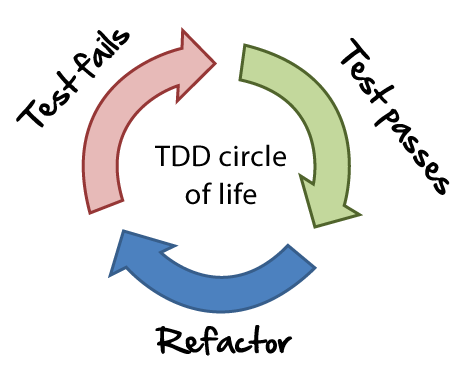
\includegraphics[scale=0.25]{sections/gestio/tdd_circle.png}
\centering
\caption{TDD}
\label{fig:tdd}
\end{figure}
\newline La figura anterior ens mostra el cicle de vida de \textit{TDD}, format per les tres fases anteriorment esmentades:
\begin{enumerate}
    \item Vermell, abans de la funcionalitat s'ha de desenvolupar el test i fer que falli
    \item Verd, es desenvolupa la funcionalitat i passa els testos
    \item Blau, refactoritzar el codi
\end{enumerate}
El seguir aquest \textit{workflow} té dos grans avantatges:
\begin{itemize}
    \item Primerament, el codi queda testejat, i es poden detectar errors en el comportament de cara  futurs canvis.
    \item Desenvolupar el test abans que la pròpia funcionalitat fa que mentalment el codi quedi estructurat i es contemplin casos d'ús, que normalment passarien per alt.
\end{itemize}